% ****** Start of file apssamp.tex ******
%
%   This file is part of the APS files in the REVTeX 4.1 distribution.
%   Version 4.1r of REVTeX, August 2010
%
%   Copyright (c) 2009, 2010 The American Physical Society.
%
%   See the REVTeX 4 README file for restrictions and more information.
%
% TeX'ing this file requires that you have AMS-LaTeX 2.0 installed
% as well as the rest of the prerequisites for REVTeX 4.1
%
% See the REVTeX 4 README file
% It also requires running BibTeX. The commands are as follows:
%
%  1)  latex apssamp.tex
%  2)  bibtex apssamp
%  3)  latex apssamp.tex
%  4)  latex apssamp.tex
%
\documentclass[%
 reprint,
%superscriptaddress,
%groupedaddress,
%unsortedaddress,
%runinaddress,
%frontmatterverbose,
%preprint,
%showpacs,preprintnumbers,
%nofootinbib,
%nobibnotes,
%bibnotes,
amsmath,amssymb,
%aps,
pra,
%prb,
%rmp,
%prstab,
%prstper,
%floatfix,
]{revtex4-1}

\usepackage{tabularx}
\usepackage{siunitx}
\usepackage{graphicx}% Include figure files
\usepackage{dcolumn}% Align table columns on decimal point
\usepackage{bm}% bold math
%\usepackage{hyperref}% add hypertext capabilities
%\usepackage[mathlines]{lineno}% Enable numbering of text and display math
%\linenumbers\relax % Commence numbering lines

%\usepackage[showframe,%Uncomment any one of the following lines to test
%%scale=0.7, marginratio={1:1, 2:3}, ignoreall,% default settings
%%text={7in,10in},centering,
%%margin=1.5in,
%%total={6.5in,8.75in}, top=1.2in, left=0.9in, includefoot,
%%height=10in,a5paper,hmargin={3cm,0.8in},
%]{geometry}

\begin{document}

\preprint{APS/123-QED}

\title{Fabrication and characterization of a Pseudo-MOSFET}% Force line breaks with \\

\author{Moritz Berger}
 \altaffiliation[]{RWTH Aachen University, Germany}%Lines break automatically or can be forced with \\
 \email{moritz.berger@rwth-aachen.de}
 \author{Gerald Kolter}
 \altaffiliation[]{RWTH Aachen University, Germany}%Lines break automatically or can be forced with \\
 \email{gerald.kolter@rwth-aachen.de}

\date{\today}% It is always \today, today,
             %  but any date may be explicitly specified

\begin{abstract}
abstract
\end{abstract}

\maketitle


\section{Introduction}
The Pseudo-MOSFET structure is a simple test structure to determine properties of Si film/oxide \citep{Park}. \\
In the following the fabrication of a Pseudo-MOSFET ("metallic-oxide-semiconductor-field-effect-transistor") will be described. The next step is a more detailed description of optical lithographie and reactive ion etching. Afterwards an analysis and a discussion of the characterization of the fabricated Pseudo-MOSFET will be given.


\section{Fabrication}

\begin{table}
\centering
\begin{tabular}{|c|c|}
\hline 
Fabrication technology & "UNIBOND" \\ 
\hline 
top Si thickness & \SI{85}{nm} \\ 
\hline 
buried oxide thickness & \SI{145}{nm} \\ 
\hline 
doping type & p-type (Boron) \\ 
\hline 
doping concentration & $1 \times 10^{15}$ \si{\per\cubic\centi\meter} \\ 
\hline 
crystal orientation & (100) \\ 
\hline 
\end{tabular} 
\caption{Specification of the SOI wafer.}
\label{tab:Spec_SOI}
\end{table}

\begin{table}
\centering
\begin{tabular}{|c|c|}
\hline 
etchant & phosphoric acid, nitric acid, acetic acid and \\ 
 & water in a volume ratio of 16:1:1:2 \\ 
\hline 
resist & AZ701MiR \\ 
\hline 
developer & AZ 726 MIF \\ 
\hline 
energy deposition & \SI{113.1}{mJ \per\centi\meter\square} @\SI{405}{nm} \\ 
\hline 
\end{tabular} 
\caption{Specification of the lithographie used for structuring the aluminum layer.}
\label{tab:Spec_Fab_Al}
\end{table}

The basis for the MOSFET are SOI (Semiconductor On Insulator) samples, the specifications are listed in table \ref{tab:Spec_SOI}. Si is used as semiconductor and SiO$_2$ as insulator. \\
In a first step a mask for the mesa structuring was defined lithographically. The etching is done by reactive ion etching with a gas mixture of SF$_6$/O$_2$. For removing the resist an oxygen plasma is used. At next the samples are RCA-cleaned ending with a dip in hydroflourid acid to get a bare silicon surface. \SI{100}{nm} aluminum is deposited in a vacuum chamber. The aluminum layer is structured with optical lithographie and an aluminum etching. The used resist, developer, etchant and the energy deposition are listed in table \ref{tab:Spec_Fab_Al}.


\section{Theory}

\subsection{Optical Lithographie}

\begin{figure}
\centering
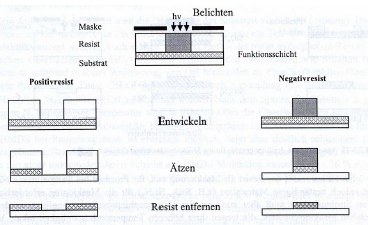
\includegraphics[scale=1.0]{Bilder/Lithographie.PNG}
\caption{Operating principle of Optical Lithographie with the different steps. Taken from \cite{Volklein00}}
\label{fig:Lithographie}
\end{figure}

The goal of optical lithographie is to deposite small structures of thin layers. In general one distinguish between two types of optical lithographie: Positiv (on the left in fig. \ref{fig:Lithographie}) and negativ (on the right in fig. \ref{fig:Lithographie}). \\
For both types the first step is to place a resist on the sample. To get a thin layer of the resist the wafer is rotated with a spin-on. Typically the lacquer has to be baked afterwards. The next step is the exposure of the resist with a mask which defines the structure to be build. To remove the resist only at the relevant parts the sample is developed. At this step the difference between positiv and negativ lithographie can be seen the first time: In positiv lithographie the resist at the exposed parts is removed and in negativ lithographie the resist at the non-exposed parts is removed. \\
Afterwards the etching is applied and the resist prevents the layer underneath at those parts where the resist was not removed. As last step the remaining resist has to be removed.


\subsection{Reactive Ion Etching}

\begin{figure}
\centering
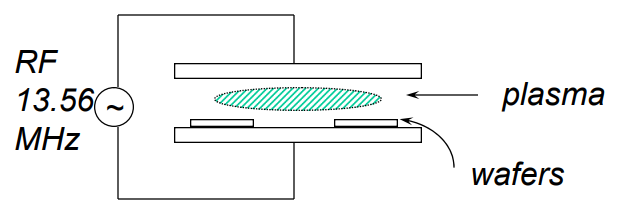
\includegraphics[scale=0.5]{Bilder/Reactive_Ion_Etching.PNG}
\caption{Setup for Reactive Ion Etching. Taken from \cite{Cheung}}
\label{fig:Reactive_Ion_Etching}
\end{figure}

The general setup for reactive ion etching is shown in fig. \ref{fig:Reactive_Ion_Etching}: In a vacuum chamber a capacitor with an oszillating electric field is placed. The wafer gets placed on one electrode. The frequency used is $f = \SI{13.56}{MHz}$. The reason is to not get interference with frequencies used for radio outside the laboratory. \\
After the vacuum has established the etching gas is released in the chamber. The fast oszillating strong electric field establishes a plasma separating the electrons and ions of the etching gas. \\
With switching from the oszillating to a static electric field the ions get accalerated towards the electrode on which the wafer is. The ions react with the material to be etched and this way the material is removed. \\
After the reactive ion etching an O$_2$ plasma is used to remove the resist.


\section{Data Analysis}

\subsection{Measurement}
On the wafer are multiple devices with different sizes. For one of these the output characteristic is measured via measuring the drain source current for different gate voltages at constant drain source voltage. \\
Afterwards for multiple devices the transfer characteristic is measured. This is done by measuring the drain source current for different drain source voltages at constant gate voltage.


\subsection{Data}

\begin{figure}
\centering
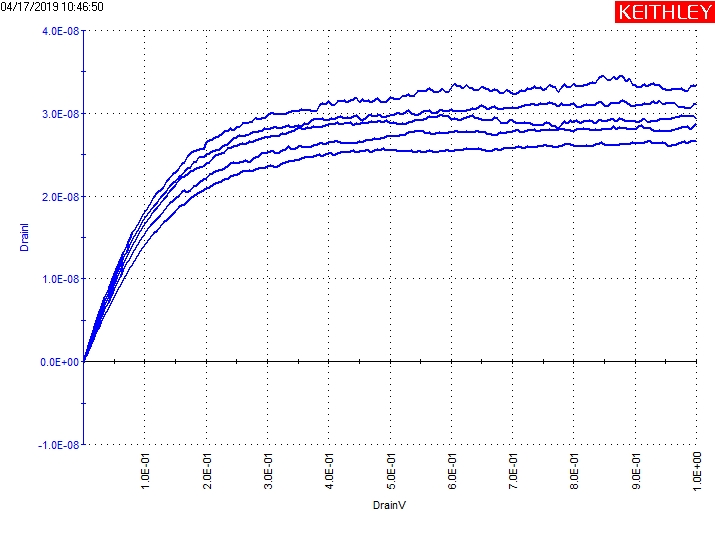
\includegraphics[scale=0.5]{Bilder/output_4c3.PNG}
\caption{Output characteristic}
\label{fig:output_4c3}
\end{figure}

\begin{figure}
\centering
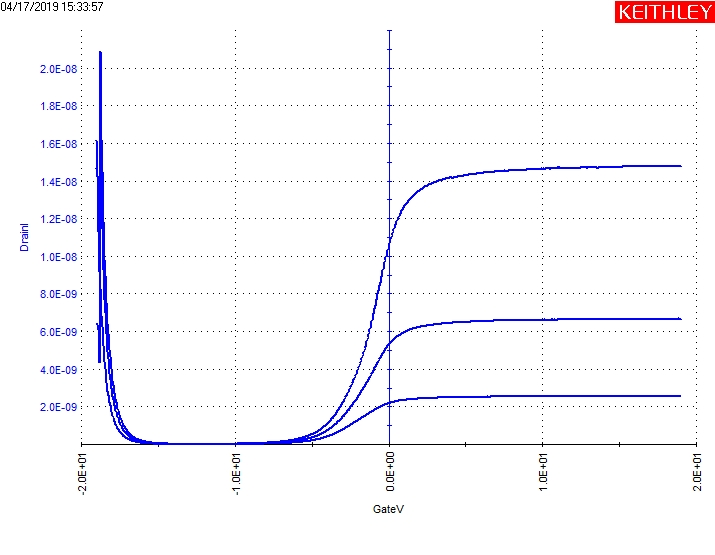
\includegraphics[scale=0.5]{Bilder/transfer_1d2.PNG}
\caption{Transfer charateristic}
\label{fig:transfer_1d2}
\end{figure}

Fig. \ref{fig:output_4c3} shows the measured output characteristic for one of the devices. As expected at low drain source voltages the drain source current raises linearly until it saturates. \\
Fig \ref{fig:transfer_1d2} shows the measured transfer characteristic for one of the devices. In principle this plot shows a similar behaviour of the transfer characteristic as the output characteristic. At very negativ gate voltages one can see, that the drain source current is rising again. This effekt is called ambipolarity.


\section{Results and Discussion}

\section{Conclusion}

\bibliography{MOSFET}% Produces the bibliography via BibTeX.

\end{document}
